\documentclass{beamer}

% Präsentationseinstellungen
\usetheme{Boadilla}
\usecolortheme{rose}
\usepackage{mathtools}
\usepackage{dsfont}
\everymath{\displaystyle}
\usefonttheme[onlymath]{serif}
\beamertemplatenavigationsymbolsempty

\DeclareMathOperator\arcosh{arcosh}
\DeclareMathOperator\Spur{Spur}

\newcommand{\1}{\mathds{1}}
\newcommand{\dt}{\;\mathrm{d}t}
\newcommand{\dx}{\;\mathrm{d}x}
\newcommand{\Cinfty}{\mathcal{C}^{\infty}}
\newcommand{\im}{\text{Im}}
\newcommand{\C}{\mathbb{C}}
\newcommand{\E}{\mathbb{E}}
\newcommand{\K}{\mathbb{K}}
\newcommand{\N}{\mathbb{N}}
\newcommand{\R}{\mathbb{R}}
\newcommand{\SR}{\mathcal{S}}

\renewcommand{\mid}{\;\middle|\;}

\title{Spektraldichte großer Matrizen}
\subtitle{Eine numerische Annäherung}
\author{Carina Seidel}
\institute[Universität Potsdam]{Universität Potsdam}
\date[3. Juli 2024]{3. Juli 2024}
\logo{
\includegraphics[height = 1.5cm]{Uni Potsdam.png}}

\begin{document}

\begin{frame}
\titlepage
\end{frame}
\begin{frame}
\frametitle{Inhaltsverzeichnis}
\tableofcontents
\end{frame}

\section{Einleitung}

\begin{frame}
    \frametitle{Motivation}
    \begin{itemize}
        \item Eigenwerte einer Matrix sind in vielen Bereichen der Mathematik und Physik interessant
        \item Oftmals sind Matrizen zu groß um diese effizient zu berechnen
        \item Stattdessen berechnen wir die Spektraldichte (Density of States)
    \end{itemize}
\end{frame}

\begin{frame}
    \frametitle{Delta Distribution}
    Sei $\mathcal{E} = \Cinfty(\Omega)$ mit $0 \in \Omega \subset \K^n$\\
    Dann ist $\delta: \mathcal{E} \to \K, f \mapsto f(0)$ mit $\delta(f) = \langle \delta, f \rangle = f(0)$\\
    Wichtige Eigenschaft:
    $$\int\limits_{-\infty}^{\infty} f(x) \delta(x-a) \dx = \int\limits_{-\infty}^{\infty} f(x) \delta(a-x) \dx = f(a) \implies \int\limits_{-\infty}^{\infty} \delta(x-a) = 1$$
\end{frame}

% \begin{frame}
%     \frametitle{Trägheitssatz von Sylvester}
%     Sei $V$ ein endlich-dimensionaler Vektorraum über $\C$.\\
%     Sei $s: V \times V \to \C$ eine hermitesche Sesquilinearform\\
%     Sei außerdem $V_0 := \{v \in V: (\forall w \in V) \; s(v,w) = 0\}$ sowie\\
%     $V_{+} := \{v \in V: s(v,v) > 0\}$ und $V_{-} := \{v \in V: s(v,v) < 0\}$\\
%     Dann gilt $$V = V_{+} \oplus V_{-} \oplus V_0$$
%     Hieraus folgt für $A \in \R^{n \times n}$ und $S \in GL(n, \R)$, dass $A$ und $S^TAS$ mit Vielfachheit gezählt die gleichen Anzahlen positiver und negativer Eigenwerte haben.
% \end{frame}

\begin{frame}
    \frametitle{Spektraldichte}
    Sei $A \in \R^{n \times n}$, $A^T = A$ und $A$ spärlich besetzt.\\
    Dann ist die Spektraldichte (engl. Denisty of States (DOS)) definiert als 
    \begin{equation}
        \phi(t) = \frac{1}{n} \sum_{j=1}^{n} \delta(t - \lambda_j)
    \end{equation}
    wobei $\delta$ die Dirac Verteilung und $\lambda_j$ die Eigenwerte von A in nicht-absteigender Reihenfolge sind.\\
    Die Anzahl der Eigenwert in einem Intervall $[a, b]$ kann dann wie folgt ausgedrückt werden:
    \begin{equation} \label{eq:nuab}
        \nu_{[a, b]} = \int\limits_a^b \sum \delta(t - \lambda_j) \dt \equiv \int\limits_a^b n \phi(t) \dt
    \end{equation}
\end{frame}

\begin{frame}
    \frametitle{Problemstellung}
    \begin{itemize}
        \item Spektraldichte trivial wenn Eigenwerte von A bekannt
        \item Unpraktisch wenn A sehr groß, da Berechnung teuer
        \item Wir brauchen effiziente Alternativen um $\phi(t)$ abzuschätzen
        \item Allerdings: $\phi(t)$ keine "Funktion" im eigentlichen Sinne
    \end{itemize}
\end{frame}

\begin{frame}
    \frametitle{Idee}
    \begin{itemize}
        \item Sei $I \subseteq \R$ das Interval, dass das Spektrum von $A$ beinhaltet.
        \item Teile nun $I$ in kleinere Teilintervalle $[t_i, t_{i+1}]$
        \item Benutze den Silvestreschen Trägheitssatz um die Eigenwerte in jedem Teilintervall zu zählen.
        \item Berechne den Durchschnittswert von $\phi(t)$ in jedem dieser Intervalle mithilfe von %\eqref{eq:nuab}
        \item Für $(t_{i+1} - t_i) \longrightarrow 0$ nähern sich die Histogramme der Spektraldichte.
        \item Problem: Berechnung der Zerlegung $A - t_i I = LDL^T$ für alle $t_i$ ist zu zeitaufwendig.
        \item Besser: $A$ nur mit Vektoren multiplizieren.
    \end{itemize}
\end{frame}

\begin{frame}
    \frametitle{Annahmen}
    \begin{itemize}
        \item Wir betrachten zwei Methoden zur Annäherung der Spektraldichte
        \item Der Einfachheit halber sei im Folgenden immer $A \in \R^{n \times n}$, $A^T = A$
        \item Die Verallgemeinerung auf hermitesche Matrizen ist im Nachhinein unkompliziert
        \item Zunächst die Kernel-Polynom-Methode (KPM)
        \item Danach das klassische Lanczos-Verfahren zur teilweisen Diagonalisierung von A
        \item Schwierig zu beurteilen welche Methode die beste ist
    \end{itemize}
\end{frame}

\begin{frame}
    \frametitle{Kernel-Polynom-Methode (KPM)}
    \begin{itemize}
        \item Formelle polynomiale Erweiterung der Spektraldichte.
        \item Macht von der Moment Matching Methode gebrauch.
        \item Wir zeigen, wie das Lanczos-Spektrokopieverfahren mit der KPM zusammenhängt
        \item Eine weitere Variante ist die Delta-Gauss-Legendre Methode
    \end{itemize}
\end{frame}

\section{Die Kernel-Polynom-Methode}

\begin{frame}
    \frametitle{Einführung}
    \begin{itemize}
        \item Zwei Klassen, KPM und Lanczos-Spektrokopieverfahren
        \item Zwei Methoden sind äquivalent zur KPM
        \item Die andere Klasse basiert auf der partiellen Tridiagonalisierung
        \item Zwei Methoden, Gaußscher und Lorentzscher Weichzeichnung (Regularisierung)
        \item Alle Methoden benutzen eine stochastische Sampling-Methode, die auf folgendem Resultat basiert:
    \end{itemize}
\end{frame}

\begin{frame}
    \frametitle{Theorem}
    Sei $A \in \R^{n \times n}$ mit Spektralzerlegung $A = \sum_{j = 1}^n \lambda_j u_j u_j^T$ wobei $u_iu_j^T = \delta_{ij}$.\\
    Sei außerdem $v \in \R^n$ mit $v = \sum_{j=1}^n \beta_j u_j$\\
    Gilt $v_i \sim \mathcal{N}(0, 1)$ i.i.d. für die Komponenten $\{v_i\}_{i = 1}^n$ von $v$, also $\E[v] = 0$ und $\E[vv^T] = \1_n$, dann
    $$\E[\beta_i \beta_j] = \delta_{ij}, \quad i,j \in \N_1^n$$
\end{frame}

\begin{frame}
    \frametitle{Beweisskizze}
    \begin{proof}[Beweis Theorem 1]
        Für $U = \left[u_1, u_2, \dots, u_n\right]$ und $\beta = \left(\beta_1, \beta_2, \dots, \beta_n\right)^T$ gilt $v = U \beta$\\
        Daher folgt, dass
        $$\E[v] = \E[U\beta] = U\E[\beta] = 0 \implies \E[\beta] = 0$$
        Weiterhin gilt, dass
        $$\E[vv^T] = \E[(U\beta)(U\beta)^T] = \E[U\beta \beta^TU^T] = U \E[\beta \beta^T]U^T = \1_n$$
        woraus folgt, dass $\E[\beta \beta^T] = \1_n$
    \end{proof}
\end{frame}

\begin{frame}
    \frametitle{Resultat}
    Sei $f(A)$ eine Matrixfunktion. Dann haben wir 
    \begin{align*}
        \E\left[v^Tf(A)v\right] & = \E\left[(U\beta)^Tf(U\Lambda U^T)(U\beta)\right]\\
        & = \E\left[\beta^TU^TUf(\Lambda)U^TU\beta\right]\\
        & = \E\left[\beta^Tf(\Lambda)\beta\right]\\
        & = \E\left[\sum_{j = 1}^n \beta_j^2 f(\lambda_j) \right]\\
        & = \sum_{j = 1}^n f(\lambda_j) \E\left[ \beta_j^2 \right]\\
        & = \sum_{j = 1}^n f(\lambda_j)
    \end{align*}
\end{frame}

\begin{frame}
    \frametitle{Tschebyschev-Polynome}
    Mit Hilfe der trigonometrischen Funktionen können die Tschebyschev wie folgt ausgedrückt werden:
    \[ T_k(t) =
    \begin{cases}
        \cos(k \arccos(t))            & \quad \text{für } k \in [-1, 1]\\
        \cosh(k \arcosh(t))           & \quad \text{für } k > 1\\
        (-1)^k \cosh(k \arcosh(-t))   & \quad \text{für } k < -1
    \end{cases}
    \]
    Es gilt außerdem die Rekursionsformel
    $$T_{k + 1}(t) = 2tT_k(t) - T_{k - 1}(t)$$
\end{frame}

\begin{frame}
    \frametitle{Transformation der Eigenwerte}
    Wir benutzen im Folgenden $T_k(t) = \cos(k \arccos(t))$ um die Dirac-Dichte zu erweitern.\\
    Wir müssen uns daher auf Matrizen beschränken, deren Eigenwerte im Intervall $[-1, 1]$ liegen.\\
    Seien daher $\lambda_{us}$ und $\lambda_{os}$ jeweils die untere bzw. obere Schranke für die Eigenwerte von $A$.
    Definiere
    $$c := \frac{\lambda_{us} + \lambda_{os}}{2} \quad \text{und} \quad d := \frac{\lambda_{os} - \lambda_{us}}{2}$$
    Dann ist $B = \frac{A - c*\1_n}{d}$ eine Matrix mit Eigenwerten im Intervall $[-1, 1]$
\end{frame}

\begin{frame}
    \frametitle{Erweiterung der Delta-Distribution}
    Berechne zunächst
    $$\hat{\phi}(t) = \sqrt{1 - t^2} \phi(t) = \sqrt{1 - t^2} \times \frac{1}{n} \sum_{j = 1}^n \delta(t - \lambda_j)$$
    Nun erweitern wir
    $$\hat{\phi}(t) = \sum_{k = 0}^{\infty} \mu_k T_k(t)$$
    im Sinne von
    $$\int \limits_{-1}^1 \hat{\phi}(t) g(t) \dt = \int \limits_{-1}^1 \sum_{k = 0}^{\infty} \mu_k T_k(t) g(t) \dt$$
    für $g \in \SR$
\end{frame}

\begin{frame}
    \frametitle{Momentenmethode}
    \begin{align*}
        \mu_k &= \frac{2 - \delta_{k0}}{\pi} \int\limits_{-1}^1 \frac{1}{\sqrt{1 - t^2}} T_k(t) \hat\phi(t) \dt\\
        &= \frac{2 - \delta_{k0}}{\pi} \int\limits_{-1}^1 \frac{1}{\sqrt{1 - t^2}} T_k(t) \sqrt{1 - t^2} \phi(t) \dt\\
        &= \frac{2 - \delta_{k0}}{n \pi} \sum_{j = 1}^n T_k(\lambda_j)\\
        &= \frac{2 - \delta_{k0}}{n \pi} \Spur(T_k(A))
    \end{align*}
\end{frame}

\begin{frame}
    \frametitle{Weitere Parameter}
    Es folgt, dass
    $$\zeta_k = \frac{1}{n_{vec}} \sum_{l = 1}^{n_{vec}} \left( v_0^{(l)} \right)^T T_k(A) v_0^{(l)}$$
    ein guter Schätzer für $\Spur(T_k(A))$ ist und damit
    $$\mu_k \approx \frac{2 - \delta_{k0}}{n \pi} \zeta_k$$
\end{frame}

\begin{frame}
    \frametitle{Berechnung der $\zeta_k$}
    Sei im Folgenden $v_0 \equiv v_0^{(l)}$
    Berechne nun
    $$T_{k + 1}(A)v_0 = 2 A T_k(A) v_0 - T_{k - 1}(A) v_0$$
    Für $v_k \equiv T_k(A)v_0$ gilt also, dass
    $$v_{k + 1} = 2 A v_k - v_{k - 1}$$
\end{frame}

\begin{frame}
    \frametitle{Definition $\tilde{\phi}_M(t)$}
    Sobald die $\{ \mu_k \}$ bestimmt sind, wäre die Erweiterung theoretisch durch
    $$\phi(t) = \frac{1}{\sqrt{1 - t^2}} \hat{\phi}(t)$$
    gegeben. Allerdings gilt
    $$\lim \limits_{k \to \infty} \mu_k \to 0$$
    und wir interessieren uns nur für $T_k(t)$ mit $k \leq M$\\
    Daher schätzen wir $\phi$ durch
    $$\tilde{\phi}_M(t) = \frac{1}{\sqrt{1 - t^2}} \sum_{k = 0}^{M} \mu_k T_k(t)$$
\end{frame}

\section{Qualitätsanalyse der Annäherungen}

\begin{frame}
    \frametitle{Problemstellung}
    \begin{itemize}
        \item Sei im Folgenden $\tilde{\phi}(t)$ eine reguläre Funktion die die Spektraldichte schätzt
        \item Alle Annäherungen sind stetige Funktionen
        \item $\phi(t)$ ist keine Funktion im eigentlichen Sinne
        \item Wir können nicht die $L^p$-Norm benutzen, um $\phi(t) - \tilde{\phi}(t)$ abzuschätzen
        \item Zwei Möglichkeiten, dies zu umgehen
    \end{itemize}
\end{frame}

\begin{frame}
    \frametitle{Schwartz-Raum über $\R$}
    $$\SR(\R) := \left\{f \in \Cinfty(\R) \mid \forall p, k \in \N_0: \sup_{x \in \R} \left| x^pf^{(k)}(x)\right| < \infty \right\}$$
\end{frame}

\begin{frame}
    \frametitle{Erste Methode}
    Wir benutzen die Tatsache, dass $\delta(t)$ eine Verteilung ist:\\
    Sei $g \in \Cinfty(\R)$ eine Testfunktion aus dem Schwartz-Raum $\SR$, dann
    $$\langle \delta(\cdot - \lambda), g \rangle \equiv \int\limits_{-\infty}^{\infty} \delta(t - \lambda) g(t) \dt \equiv g(\lambda)$$
    und für alle $p, k \in \N_0$ $$\sup_{t \in \R} |t^pg^{(k)}(t)| < \infty$$
    Dann wird der Fehler wie folgt gemessen: $$\epsilon_1 = \sup_{g \in \SR} \left| \langle \phi, g \rangle - \langle \tilde{\phi}, g \rangle \right|$$
\end{frame}

\begin{frame}
    \frametitle{Zweite Methode}
    Wir "regularisieren" die $\delta(t)$-Funktionen\\
    Dazu ersetzen wir sie durch stetige und glatte Funktionen\\
    Zum Beispiel die Gaussche Normalverteilung mit einer angemessene Standardabweichung $\sigma$\\
    Die daraus entstandene Funktion $\phi_{\sigma}(t)$ ist wohldefiniert\\
    Für $p=1, 2$ und $\infty$ können wir folgenden Fehler berechnen:
    \begin{equation} \label{eq:eps2}
        \epsilon_2 = \left|\left| \phi_{\sigma}(t) - \tilde{\phi}(t) \right|\right|_p
    \end{equation}
    Diese beiden Methoden sind eng verwandt!
\end{frame}

\begin{frame}
    \frametitle{Der Begriff der Auflösung}
    Selten ist eine exakte Annäherung aller Eigenwerte von $A$ gewünscht.\\
    Oftmals genügt es, die Anzahl der Eigenwerte in einem beliebigen Teilintervall $[a, b]$ des Spektrums zu wissen.\\
    Die Größe $b - a$ dieses Teilintervalls bezeichnet man als Auflösung der Schätzung:\\
    Je kleiner das Teilintervall, desto höher die Auflösung.\\
    Die Genauigkeit der Annäherung ist nur bis zur gewünschten Auflösung aussagekräftig.\\
    Für $\epsilon_2 = \left|\left| \phi_{\sigma}(t) - \tilde{\phi}(t) \right|\right|_p$ aus \eqref{eq:eps2} gilt:\\
    Je kleiner das $\sigma$, desto höher die Auflösung.
\end{frame}

\begin{frame}
    \frametitle{Noch mehr Probleme mit Dirac}
    Betrachte
    $$\nu_{[a, b]} = \int\limits_a^b n \phi(t) \dt$$
    aus \eqref{eq:nuab}. Definiere entsprechend
    $$\tilde{\nu}_{[a, b]} = \int\limits_a^b n \tilde{\phi(t)} \dt$$
    mit $\tilde{\phi}(t) \in \Cinfty$
\end{frame}

\begin{frame}
    \frametitle{Noch mehr Probleme mit Dirac (2)}
    Angenommen, $n = 1$ und $\phi(t) = \delta(t)$.\\
    Unendliche Auflösung bedeutet $\left| \nu_{[a, b]} - \tilde{\nu}_{[a, b]} \right|$ soll für $[a ,b]$ beliebig klein ebenfalls klein sein.\\
    Sei also $a = -\varepsilon, b = \varepsilon$. Aus der Definition der $\delta$-Funktion folgt dann, dass
    $$\lim \limits_{\varepsilon \to 0+} \nu_{[-\varepsilon, \varepsilon]} = 1$$
    während für glatte Funktionen $\tilde{\phi}$ selbstverständlich gilt, dass
    $$\lim \limits_{\varepsilon \to 0+} \tilde{\nu}_{[-\varepsilon, \varepsilon]} = 0$$
    Fazit: Keine glatte Funktion konvergiert zur Spektraldichte unter stetiger Erhöhung der Auflösung
\end{frame}

\begin{frame}
    \frametitle{Einschränkung des Schwartz-Raums}
    Eine endliche Auflösung ist oftmals genug.\\
    Wir können den Schwartz-Raum $\SR$ also einschränken.\\
    Beispiel: Betrachte nur Gaussche Verteilungsfunktionen der Form
    $$g_{\sigma}(t) = \frac{1}{(2\pi\sigma^2)^\frac{1}{2}}e^{-\frac{t^2}{2\sigma^2}}$$
    und schränke $\SR$ auf den Unterraum
    $$\SR(\sigma;[\lambda_{lb}, \lambda_{ub}]) = \left\{ g \mid g(t) \equiv g_{\sigma}(t - \lambda), \lambda \in [\lambda_{lb}, \lambda_{ub}] \right\}$$
    Hierbei sind $\lambda_{lb}$ und $\lambda_{ub}$ jeweils das Infimum und Supremum der Eigenwerte von $A$ und der Parameter $\sigma$ die \emph{Zielauflösung}.\\
    Wir können nun die folgende Metrik zur Qualitätsbewertung nutzen:
    \begin{equation} \label{eq:error}
        E\left[\tilde{\phi};\SR\left(\sigma; \left[\lambda_{lb}, \lambda_{ub} \right] \right)\right] = \sup_{g \in \SR(\sigma;[\lambda_{lb}, \lambda_{ub}])} \left| \langle \phi, g \rangle - \langle \tilde{\phi}, g \rangle \right|
    \end{equation}
\end{frame}

\begin{frame}
    \frametitle{Regularisierung der Spektraldichte}
    \begin{itemize}
        \item Konstruiere zunächst eine glatte Darstellung der $\delta$-Funktion.
        \item Dies muss verhältnismäßig zur gewünschten Auflösung sein.
        \item Der Fehler kann dann direkt berechnet werden
        \item Wahl des $\sigma$: so groß wie möglich für leichte Annäherung, so klein wie möglich für Genauigkeit
    \end{itemize}
\end{frame}

\begin{frame}
    \frametitle{Regularisierung der Spektraldichte mit Gauss}
    Sei $$\phi_{\sigma}(t) = \left \langle \phi(\cdot), g_{\sigma}(\cdot - t)\right \rangle = \sum_{j = 1}^n g_{\sigma}(t - \lambda_j)$$
    Dies ist dann nicht anderes als die "Weichzeichnung" der Spektraldichte durch Gauß-Funktionen der Breite $\sigma$\\
    Genauso sei $$\tilde{\phi}_{\sigma}(t) = \langle \tilde{\phi}(\cdot), g_{\sigma}(\cdot - t) \rangle$$
    Dann ist
    $$E\left[\tilde{\phi};\SR\left(\sigma; \left[\lambda_{lb}, \lambda_{ub} \right] \right)\right] = \sup_{g \in \SR(\sigma;[\lambda_{lb}, \lambda_{ub}])} \left| \langle \phi(\cdot), g_{\sigma}(\cdot - t) \rangle - \langle \tilde{\phi}(\cdot), g_{\sigma}(\cdot - t) \rangle \right|$$
    der $L^\infty$-Fehler zwischen zwei wohldefinierten Funktionen
\end{frame}

\begin{frame}
    \frametitle{Schöne Bilder}
    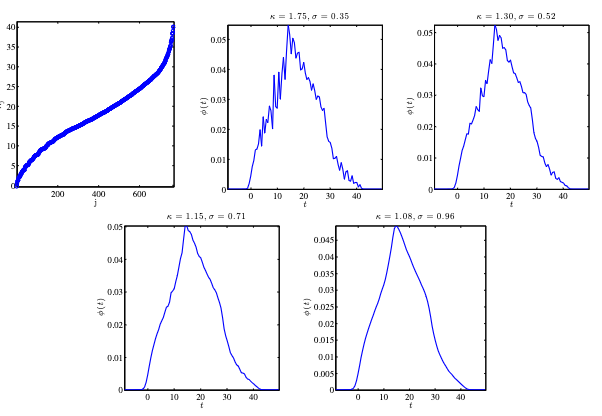
\includegraphics[height=7.5cm]{screenshot.png}
\end{frame}

\begin{frame}
    \frametitle{Regularisierung der Spektraldichte mit Lorentz}
    Die Lorentz-Funktion ist definiert durch
    $$\frac{\eta}{(t - \lambda)^2 + \eta^2} = -\im \left( \frac{1}{t - \lambda + i \eta} \right) \; ,$$
    wobei $\eta$ eine kleine Regularisierungskonstante ist.\\
    Für $\eta \to 0$ nähert sich die Lorentz-Funktion der Dirac-Funktion um den Eigenwert $\lambda$ an\\
    Dies ist später für die Haydock-Methode relevant.
\end{frame}

\begin{frame}
    \frametitle{Die Bedingung der Nicht-Negativität}
    \begin{itemize}
        \item Die Spektraldichte ist als Wahrscheinlichkeitsverteilung nicht-negativ, also
        $$\forall g \in \SR, g \geq 0: \langle \phi, g \rangle \geq 0$$
        \item Einige numerische Annäherungen brechen mit dieser Eigenschaft
        \item Das führt zu großen Fehlern
    \end{itemize}
\end{frame}

\section{Auswertung}

\end{document}